% !TEX root = ../patchEmbeddings_review.tex

\begin{figure}[t]
\centering
        % \includegraphics[width=0.4\textwidth,trim=0.25in 0.25in 0.68in 0.36in,clip]{./figs/SSBM_experiments.pdf} % 0.45
        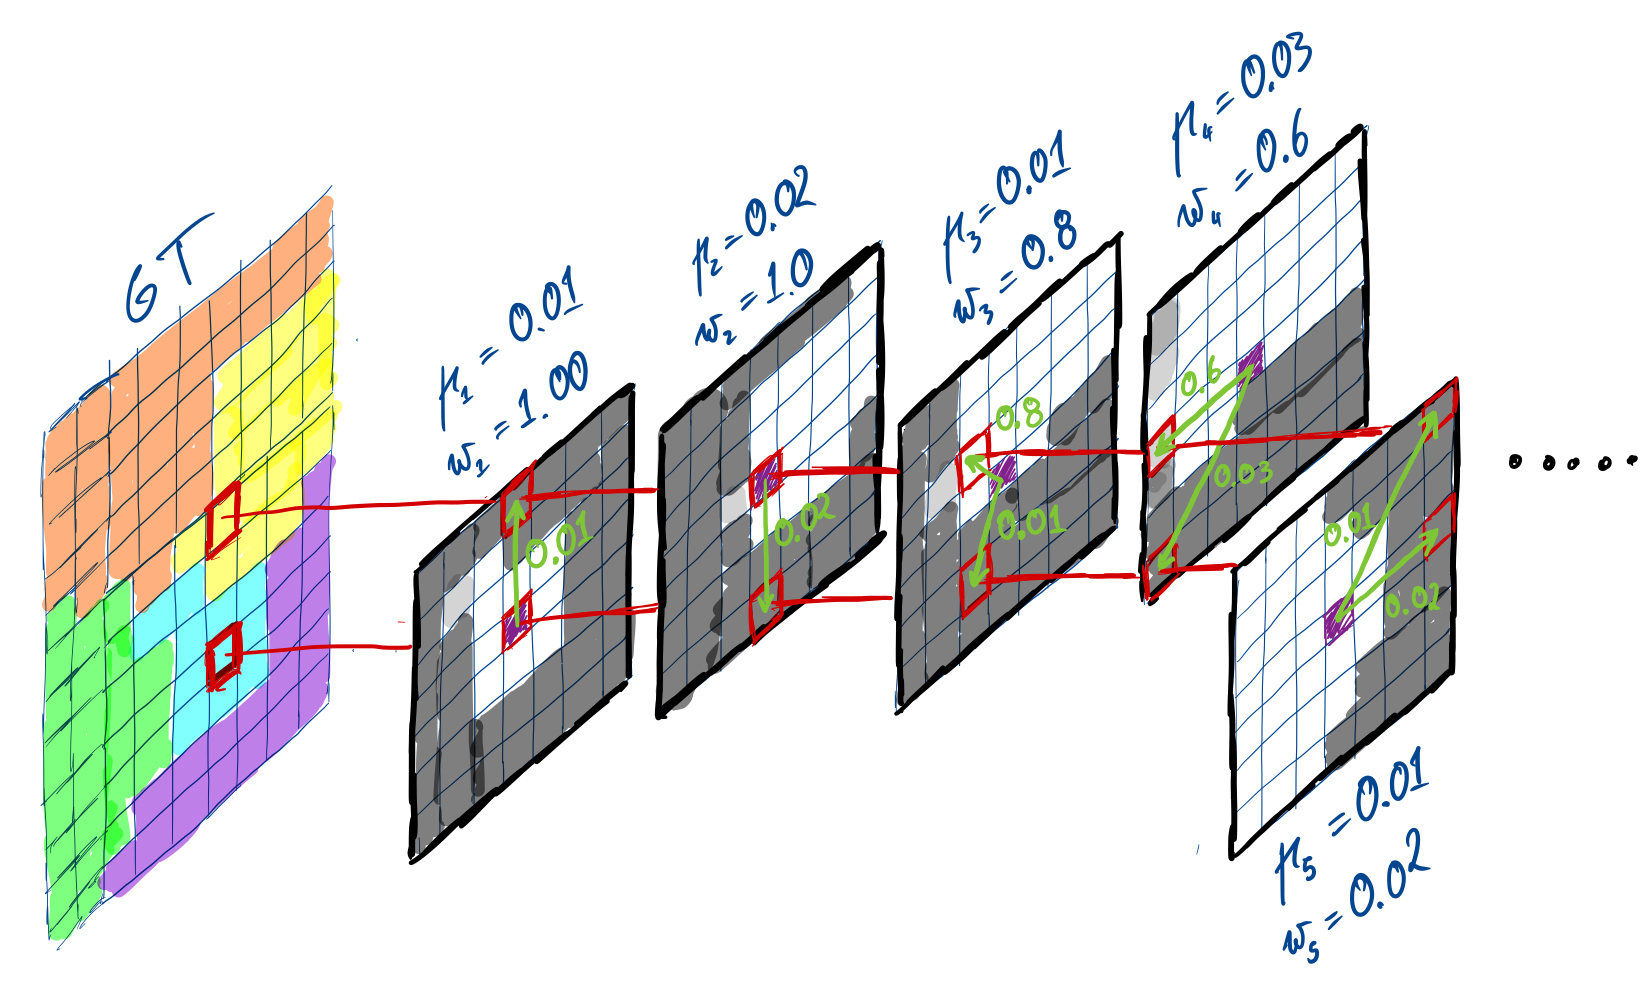
\includegraphics[width=0.7\textwidth]{./figs/alg_explaned.jpg} % 0.45
        \caption{\TODO{Update fig}  Illustration of the proposed parameter-free method to convert \maskname masks to edge weights...}
    \label{fig:alg_explained}
\end{figure}
\begin{algorithm}[t]
  \begin{flushleft}
  \caption{: Affinities from aggregated \maskname masks}
   \hspace*{\algorithmicindent} \textbf{Input:} Graph $\mathcal{G}(V,E)$; \maskname masks $\mathcal{M}_{\coord{u}}: \mathcal{N}_{K\times K} \rightarrow [0,1]$  \\
  \hspace*{\algorithmicindent} \textbf{Output:} Affinities $\bar{a}_e\in[0,1]$ with variance $\sigma^2_e$ for all edges $e\in E$\\
  \hspace*{\algorithmicindent} 
  \begin{algorithmic}[1]
  \footnotesize
  % \small
      % \State Initial clustering: $\Pi=\{\{v_1\}, \ldots, \{v_{|V|}\}\}$
      % \State Initialize interactions between clusters with $ = w^+_e - w^-_e$
      \For{each edge $e\in E$ in graph $\mathcal{G}$}
        \State Get coordinates $\coord{u}=(u_x,u_y)$ and $\coord{v}=(v_x,v_y)$ of pixels linked by edge $e$
        \State Collect all $T$ masks $\mathcal{M}_{\coord{c}_1},\ldots,\mathcal{M}_{\coord{c}_T}$ including both pixel $\coord{u}$ and pixel $\coord{v}$
        \State Init. vectors $[a_1,\ldots,a_T]$ and $[\evidW_1,\ldots,\evidW_T]$ for affinities and evidence weights
        \For{each mask $\mathcal{M}_{\coord{c}_i}$}
            \State Get relative coords. of $\coord{u}$ and $\coord{v}$ with respect to the central pixel $\coord{c}_i$
            \State $a_i \gets \min \big(\mathcal{M}_{\coord{c}_i}(\coord{u} - \coord{c}_i), \,\mathcal{M}_{\coord{c}_i}(\coord{v} - \coord{c}_i)\big)$ \Comment{Fuzzy-AND: both values active}
            \State $\evidW_i \gets \max \big(\mathcal{M}_{\coord{c}_i}(\coord{u} - \coord{c}_i), \,\mathcal{M}_{\coord{c}_i}(\coord{v} - \coord{c}_i)\big)$ \Comment{Fuzzy-OR: at least one value active}
        \EndFor
        \State Get weighted affinity average $\bar{a}_e= \sum_{i} a_i \evidW_i\,/\,\sum_{i}\evidW_i$ 
        \State Get weighted affinity variance $\sigma^2_e = \sum_{i} \evidW_i (a_i-\bar{a}_e)^2\,/\,\sum_{i}\evidW_i$
      \EndFor
      \State
      \Return $a_e, \sigma^2_e$ for each $e\in E$
  \end{algorithmic}
    \label{alg:computing_affinities}
  \end{flushleft}

\end{algorithm}

\section{Extracting affinities from \maskname masks}
In order to obtain an instance segmentation from the predictions of the model presented in Sec. \ref{sec:model}, we now compute instance-aware pixel-pair affinities for a given sparse $N$-neighborhood structure (see \TODO{Appendix} for details about the used structure) and use them as edge weights of a pixel grid-graph $\mathcal{G}(V,E)$, such that each node represents a pixel / voxel of the image. The graph is then partitioned to obtain object instances.
% \TODO{Section intro} Second contribution; two ways
% In this section, we propose two ways to perform something similar and use the predicted per-pixel \maskname masks to define the edge weights of a grid-graph.



\subsection{Efficient affinities for any sparse neighborhood}\label{sec:efficient_affs}
If the model is trained only with the \emph{\sparseBr branch} shown in Fig. \ref{fig:main_figure}a, then the desired $N$-neighborhood structure defining the connectivity of the grid-graph has to be defined before training. 
On the other hand, if the model is trained with the \emph{\encBr branch} of Fig. \ref{fig:main_figure}c, then the sparse connectivity structure of the graph can be defined at prediction time, but the \maskDec in Fig. \ref{fig:main_figure}c has to be applied to each pixel of the image in order to predict the desired affinity values, given by the value of $N$ in each mask. 
Alternatively, another much more efficient method consists in predicting these affinities directly from the $Q$-dimensional latent space of the encoded masks, by stacking few additional convolutional layers that do not need to be jointly trained with the full model and only serve to convert the encoded latent space to the desired $N$ output feature maps.
% ,  predict  from the previously trained latent space feature maps $Q\times H\times W$.
In this way, the graph $N$-neighborhood structure can be defined at prediction time, but the resulting model is no more memory-consuming than one directly trained to predict only that specific neighborhood. 



\subsection{Affinities with uncertainty from aggregated masks}\label{sec:aggr_affs}
As an alternative to the efficient method proposed in Sec. \ref{sec:efficient_affs}, in this section we propose an algorithm that, without the need of any threshold parameter, aggregates predictions from overlapping \maskname masks and output edge weights with associated uncertainty.
Related work either threshold the predicted \maskname masks \cite{januszewski2018high,hirsch2020patchperpix,meirovitch2016multi} or compute Intersection over Union (IoU) scores for overlapping patches \cite{liu2016multi}. However, an advantage of predicting pixel-pair affinities / pseudo-probabilities as compared to IoU scores is that affinities can easily be translated into attractive and repulsive interactions in the grid-graph 
% i.e. edge with either positive or negative weights, 
and a parameter-free partitioning algorithm can be employed to yield instances.
% Related work in \cite{liu2016multi} aggregate \maskname masks by computing Intersection over Union (IoU) scores for overlapping patches, however these scores cannot be translated into attractive and repulsive cues of the graph, so hierarchical agglomerative clusterings 

Here, we propose a simple method to aggregate predictions from multiple patches (see Algorithm \ref{alg:computing_affinities} and Fig. \ref{fig:alg_explained}). Let us assume we want to compute the weight for an edge $e$ linking pixels $\coord{u}$ and $\coord{v}$. Then, we consider all predicted \maskname masks including both $\coord{u}$ and $\coord{v}$. For example, if $\coord{u}$ and $\coord{v}$ are direct neighbors and the predicted masks have shape $K\times K$, then there will be $K(K-1)$ masks including both pixel $\coord{u}$ and $\coord{v}.$\footnote{Note that here we ignore possible boundary effects by considering two pixels close to the image border.} 
However, not all these masks are informative: a mask $\mathcal{M}_{\coord{c}_i}$ centered at pixel $\coord{c}_i$ provides some evidence about the affinity between pixels $\coord{u}$ and $\coord{v}$ only if at least one of the two pixels belongs to the $\coord{c}_i$-mask (fuzzy OR operator \UPDATE{at line 6} in Alg. \ref{alg:computing_affinities}).
If both pixels do not belong to it, then the evidence weight $\evidW_i$ goes to zero (Fig. \ref{fig:alg_explained}c).
On the other hand, we distinguish two cases when there is evidence and at least one pixel belongs to the $\coord{c}_i$-mask: i)
both pixels belong to it (fuzzy AND operator \UPDATE{at line 7} in Alg. \ref{alg:computing_affinities}), so by transitivity we conclude they should be in the same instance and their affinity $a_i$ should tend to one (Fig. \ref{fig:alg_explained}a); 
ii) only one pixel belongs to the $\coord{c}_i$-mask and their affinity should tend to zero (Fig. \ref{fig:alg_explained}b). 

At the end, we compute a weighted average $\bar{a}_e$ and variance $\sigma^2_e$ of the collected affinities from all overlapping masks, such that masks with more evidence will contribute more in the average and the obtained variance is a measure of how consistent were the predictions across masks. 
The algorithm was implemented on GPU using PyTorch \cite{NEURIPS2019_9015} and the variance was computed via the Welford's online and stable algorithm \cite{welford1962note}.




